\documentclass{article}

\usepackage{../../austin137}
\usepackage{../../local}
\usehyperstuff

\newcommand{\basvec}[2]{\hat{#1}_{#2}}							% 	Basis vector
\newcommand{\basdual}[2]{\underline{\smash{\hat{#1}}}{}^{#2}}				% 	Dual basis vector
%\newcommand{\dual}[1]{\underline{#1}}							% 	Dual vector
\newcommand{\pascovar}[2]{C^{#1}_{\phantom{#1}#2}}					% 	Change of basis matrix
\newcommand{\pascontra}[2]{(C^{-1})^{#1}_{\phantom{#1}#2}}				% 	Change of basis matrix
\newcommand{\actcovar}[2]{(R^{-1})^{#1}_{\phantom{#1}#2}}					% 	Change of basis matrix
\newcommand{\actcontra}[2]{(R)^{#1}_{\phantom{#1}#2}}				% 	Change of basis matrix
\def\mat{(\textrm{mat})}


\def\stress{\boldsymbol{\sigma}}
\def\strain{\boldsymbol{\epsilon}}
\def\stiffness{\boldsymbol{\mathsf{C}}}
\def\comply{\boldsymbol{\mathsf{S}}}

\usepackage{wrapfig}

\begin{document}

%%%%%%%%%%%%%%%%%%%%%%%%%%%%%%%%%%%%%%%%%%%%%%%%%%%%%%%%%%%%%%%%%%%%%%%%%%%%%%%%
\addcopyright
\begin{center}
{\bf \large Physics W89 - Introduction to Mathematical Physics - Summer 2023}\\\medskip
{\bf \large Problem Set - Module 07 - This Module Makes Me Tensor} \\\medskip
{\emph{Last Update: \today}\\}
{Student: Yutong Du}
\end{center}

\dphline
%%%%%%%%%%%%%%%%%%%%%%%%%%%%%%%%%%%%%%%%%%%%%%%%%%%%%%%%%%%%%%%%%%%%%%%%%%%%%%%%
\paragraph{}
Note: In this problem set, I will be using Einstein summation convention, where all indices that are repeated - occuring once as a lower index and once as an upper index - 
are assumed to be summed over.  We will restrict ourselves to \emph{real} vector spaces for all parts of this problem set unless explicitly stated otherwise.

\dphline
\bigskip
%%%%%%%%%%%%%%%%%%%%%%%%%%%%%%%%%%%%%%%%%%%%%%%%%%%%%%%%%%%%%%%%%%%%%%%%%%%%%%%%
\section*{Problem 7.1 - Introduction to Tensors}
\relevid{An Old Acquaintance - Dual Vectors; 
Revisiting Old Friends - Vectors and Matrices;
Defining Tensors - Maps;
Defining Tensors - Components; 
The Tensor Product;
Contraction}


\paragraph{}
Consider a type-$(p,q)$ tensor $\mathsf{T}$.  We defined this as a \emph{map} or \emph{machine} that eats a set of $p$ dual vectors and $q$ vectors to return a scalar in a fully
linear fashion.  That is, if we replace any of the $p$ dual vectors or $q$ vectors with a linear combination, we can ``distribute''.  
For example, a type-(0,2) tensor $\mathsf{F}$ eats two vectors to return a scalar and satisfies
	\begin{align*}
		\mathsf{F}(c_{1}\vec{v}_{1}+c_{2}\vec{v}_{2}, \vec{w}) &= c_{1}\mathsf{F}(\vec{v_{1}},\vec{w}) + c_{2}\mathsf{F}(\vec{v}_{2},\vec{w}),\\
		\mathsf{F}(\vec{v},c_{1}\vec{w}_{1}+c_{2}\vec{w}_{2}) &= c_{1}\mathsf{F}(\vec{v},\vec{w}_{1}) + c_{2}\mathsf{F}(\vec{v},\vec{w}_{2}).
	\end{align*}
We usually define particular tensors by how exactly they act on a set of dual vectors and vectors.
For calculations involving tensors, it is useful to introduce its \emph{components}, with the components having $p$ upper indices and $q$
lower indices $T^{i_{1}\cdots i_{p}}_{[e]\!\!\!\!\!\! \phantom{i_{1}\cdots i_{p}}j_{1}\cdots j_{q}}$, defined by acting the tensor on basis elements,
	\begin{equation*}
		T^{i_{1}\cdots i_{p}}_{[e]\!\!\!\!\!\! \phantom{i_{1}\cdots i_{p}}j_{1}\cdots j_{q}} \equiv
		\mathsf{T}(\basdual{e}{i_{1}}, \cdots, \basdual{e}{i_{p}}, \basvec{e}{j_{1}}, \cdots \basvec{e}{j_{q}}).
	\end{equation*}

\phline
%%%%%%%%%%%%%%%%%%%%%
\paragraph{}
Consider a tensor $\boldsymbol{\delta}$ that eats one dual vector and one vector and whose action is to ``feed the vector to the dual vector'' to return the scalar.  That is,
	\begin{equation*}
		\boldsymbol{\delta}(\dual{\alpha},\vec{v}) \equiv \dual{\alpha}(\vec{v}).
	\end{equation*}

\paragraph{(a)}
What are the type and rank of the tensor $\boldsymbol{\delta}$?  What are the components of $\boldsymbol{\delta}$?  
Determine $\boldsymbol{\delta}(\dual{\alpha},\vec{v})$ if $\dual{\alpha}\doteq \begin{smpmatrix}{0.8} 3 & 5 & -2 \end{smpmatrix}$ 
and $\vec{v} \doteq \begin{smpmatrix}{0.7} -7 \\ 4 \\ 6\end{smpmatrix}$.
\extrasubpart{Argue that this definition is indeed linear in both its dual vector slot and its vector slot.}
\spoilerans{You should find that the components form the Kronecker delta symbol $\delta^{i}_{\ j}$!}

\begin{solution}
	Since $\delta$ eats one dual vector and a vector, it's a type (1, 1) tensor, hence its rank is 2. The 
	components of $\delta$ are determined by feeding it basis elements:
	\[
	\delta(\hat{e}^i, \hat{e}_j) = \hat{e}^i(\hat{e}_j) = \delta^i_j
	\] 
	Given $\underline\alpha$ and $\vec v$, we have:
	\[
		\delta(\underline \alpha, \vec v) = \begin{pmatrix} 3 & 5 & -2 \end{pmatrix} \begin{pmatrix} -7\\4\\6 \end{pmatrix} = -21 + 20 - 12 = -13
	\] 
\end{solution}

\phline
%%%%%%%%%%%%%%%%%%%%%
\paragraph{}
Consider a tensor $\boldsymbol{\vareps}$ that eats $n$ vectors (in an $n$-dimensional vector space) and returns the matrix determinant of the $n\times n$ matrix formed by the 
column vectors,
	\begin{equation*}
		\boldsymbol{\vareps}(\vec{v}_{1},\cdots,\vec{v}_{n}) \equiv \det\begin{pmatrix}\begin{pmatrix} \\ \vec{v}_{1}\\ \\ \end{pmatrix}_{[e]}&\cdots&
		\begin{pmatrix} \\ \vec{v}_{n}\\ \\ \end{pmatrix}_{[e]}\end{pmatrix}
		= \begin{vmatrix} (v_{1})^{1} & \cdots & (v_{n})^{1}\\\vdots & \ddots & \vdots \\ (v_{1})^{n} & \cdots & (v_{n})^{n}\end{vmatrix}.
	\end{equation*}

\paragraph{(b)}
What properties of the determinant ensure that this is a tensor?  What are the type and rank of $\boldsymbol{\vareps}$?  If we are in 3-dimensional real space 
(so $V=\mathbb{R}^{3}$ and $n=3$), what are the components of $\boldsymbol{\vareps}$?

\begin{solution}
	The determinant ``eats'' $n$ vectors, and is also fully linear in each input slot (we covered this in an 
	earlier module). These are the only two requirements needed to satisfy the fact that it is a tensor. Since
	$\epsilon$ eats $n$ vectors, it is a type (0, $n$) tensor, and hence it is also rank $n$. To find the 
	components of $\epsilon$ in 3D space, we feed it the basis vectors:
	\[
		\epsilon_{ijk} = \epsilon(\hat{e}_i, \hat{e}_j, \hat{e}_k)
	\] 
	Firstly, we know that from the properties of the determinant that if there are two identical columns, then
	the determinant is automatically zero. For us, this means that every index with a repeated component is 
	zero. For those without repeats, we first compute $\epsilon_{123}$:
	\[
		\epsilon_{123} = \det(\mathbbold 1) = 1
	\] 
	With that, now we look at how many column swaps it's required to get the other indices:
	\begin{align*}
		\epsilon_{132} &= -\epsilon_{123} = -1\\
		\epsilon_{213} &= -\epsilon_{123} = -1 \\
		\epsilon_{231} &= \epsilon_{123} = 1 && \text{since two swaps required: $123 \to 321 \to 231$}\\
		\epsilon_{321} &= -\epsilon_{123} = -1\\
		\epsilon_{312} &= \epsilon_{123} = 1 && \text{since two swaps required: $123 \to 321 \to 312$}
	\end{align*}
\end{solution}



\phline
%%%%%%%%%%%%%%%%%%%%%
\paragraph{(c)}
Determine the type of each of the following tensor combinations/actions and convert to index notation by acting your tensor on basis vectors and dual vectors:\footnote{You should
also try to guess what the index notation looks like before explicitly finding the answers.  As you get more practice you will find it easier and easier to jump between the map
and component descriptions!}
	\begin{enumerate}
		\item \heavydef{Not-for-credit example:}  $\dual{\alpha}(\vec{v}) = \alpha_{i}v^{i}$, which is a type-(0,0) object (a scalar).
		\item $\dual{\alpha}\otimes\vec{v}$, the {tensor product} of $\dual{\alpha}$ and $\vec{v}$.

			\begin{solution}
				This takes a type (1, 0) and type (0, 1) tensor to create a type (1, 1) tensor, whos index
				representation is $ \alpha_j v^i$.
			\end{solution}
		\item $\mathsf{M}(\dual{\alpha},\vec{v})$, a linear transformation $\mathsf{M}$ acting on a dual vector $\dual{\alpha}$ and a vector $\vec{v}$.

			\begin{solution}
				$M$ is a type (1, 1) tensor, and since we are acting it exactly on its ``diet'', then the result
				is a scalar, or a type (0, 0) tensor (a scalar). In index notation, it's written as:
				\[
				M(\underline \alpha, \vec v) = \alpha_i M^i_j v^j
				\] 
			\end{solution}
		\item $\mathsf{A}\otimes\mathsf{B}$, the tensor product of two linear transformations $\mathsf{A}$ and $\mathsf{B}$.

			\begin{solution}
				$A$ and $B$ are both linear transformations, hence they are both type (1, 1) tensors. Thus, 
				their tensor product creates a type (2, 2) tensor, which mas index representation $C^{i_1, i_2}_{j_1, j_2}$
			\end{solution}
		\item \heavydef{Not-for-credit example:}  Feeding a single vector $\vec{v}$ to a linear transformation, $\mathsf{M}\vec{v} \equiv \mathsf{M}(\cdot,\vec{v})$, which is
			a type-(1,0) object (a vector), with components $M^{i}_{\phantom{i}j}v^{j}$.
		\item $\mathsf{G}$, a tensor that eats two dual vectors to return a scalar.

			\begin{solution}
				Since $G$ eats two dual vectors it's a type (2, 0) tensor. As for the index notation, we should
				have two upper indices: $G^{ij}$. 
			\end{solution}
		\item $\mathsf{G}(\dual{\alpha},\cdot)$, the tensor from the previous part fed the dual vector $\dual{\alpha}$ to the first slot.

			\begin{solution}
				This tensor now requires only a single dual vector to become a scalar, hence it is a type (1, 0)
				tensor. In index notation: $G^j = \alpha_i G^{ij}$. We need the $\alpha$ here since the 
				properties of $G(\underline \alpha, \cdot)$ depend on the dual vector $\underline \alpha$ that
				we feed in.
			\end{solution}
		\item \heavydef{Not-for-credit extra part:} $\mathsf{G}(\cdot,\dual{\beta})$, the tensor from the previous part fed the dual vector $\dual{\beta}$ to the second slot.
	\end{enumerate}
\note{Detailed solutions for the not-for-credit examples (1) and (5) are given in the problem set supplement.}


\phline
%%%%%%%%%%%%%%%%%%%%%
\paragraph{}
In these next two parts we will consider type-(0,2) tensors which are the most common tensorial objects after scalars, vectors, dual vectors, and linear transformations.  
These tensors eat two vectors to return a scalar.  
First, let's restrict ourselves to a 2D vector space $V$ so that our indices can only take on two values.  A type-(0,2) tensor $\mathsf{F}$ on this space will only have $2^{2}=4$ 
components $F_{ij}$.  We can get two different dual vectors out if we feed $\mathsf{F}$ a vector $\vec{v}\doteq \vec{v}_{[e]}\equiv\smtwovect{v^{1}}{v^{2}}$ depending
on whether we plug $\vec{v}$ into the first slot or the second of $\mathsf{F}$,
\begin{align}
		\mathsf{F}(\vec{v},\cdot) &= (F_{ij}v^{i})\hat{e}_{j} \doteq \begin{pmatrix}(F_{11}v^{1} + F_{21}v^{2}) & (F_{12}v^{1}+F_{22}v^{2})\end{pmatrix},\label{Fv1}\\
		\mathsf{F}(\cdot,\vec{v}) &= (F_{ij}v^{j})\hat{e}_{i} \doteq \begin{pmatrix}(F_{11}v^{1} + F_{12}v^{2}) & (F_{21}v^{1}+F_{22}v^{2})\end{pmatrix}.\label{Fv2}
	\end{align}

Our general rule for converting index notation to matrix notation (our grids of numbers) is that upper indices label rows and lower indices label columns.  In lecture we discussed
one way to interpret an object like the type-(0,2) tensor - letting the two lower indices label two different `types' of column to give us a ``row vector of row vectors'',
	\begin{equation*}
		\mathsf{F}\doteq\mathsf{F}_{[e]} \equiv \begin{pmatrix} \begin{pmatrix} F_{11} & F_{21} \end{pmatrix} & \begin{pmatrix} F_{12} & F_{22} \end{pmatrix} \end{pmatrix}.
	\end{equation*}
While we can build a consistent method of matrix manipulations out of this, it is an uncommon practice.  Since type-(0,2) (and type-(2,0)) tensors are common objects, it
is worthwhile to review a less natural but more familiar way of dealing with these, which is to allow the first lower index to `improperly' label rows to make a matrix
form of a type-(0,2) tensor:
	\begin{equation*}
		\mathsf{F}\doteq {F}^{\mat}_{[e]} \equiv \begin{pmatrix} F_{11} & F_{12} \\ F_{21} & F_{22}\end{pmatrix}.
	\end{equation*}
\note{Remember that the objects with the subscript `$[e]$' are the matrix representations/grids of components with respect to a basis.}

\paragraph{(d)}	
Evaluate $\vec{v}_{[e]}^{\T}{F}^{\mat}_{[e]}$ and $({F}^{(\textrm{mat})}_{[e]}\vec{v}_{[e]})^{\T}$.  Show that the results are the row vector from Eqs.~\ref{Fv1} and~\ref{Fv2}, respectively.
Finally, show $\mathsf{F}(\vec{v},\vec{w}) = \vec{v}_{[e]}^{\T}{F}^{(\textrm{mat})}_{[e]}\vec{w}_{[e]}$.

\begin{solution}
	Since all objects here are nicely represented as matrices, we can just perform matrix multiplication to 
	show these properties:
	\[
		\vec v_{[e]}^\top F_{[e]}^\text{mat} = \begin{pmatrix} v^1 & v^2 \end{pmatrix} 
		\begin{pmatrix} F_{11} & F_{12}\\F_{21}& F_{22} \end{pmatrix} = \begin{pmatrix} v^1F_{11} + v^2F_{21} & 
	v^1F_{12} + v_2F_{21} \end{pmatrix}
	\]
	which equals equation 1. Now for the other one:
	\[
		(F_{[e]} \vec v_{[e]})^\top = \left[ \begin{pmatrix} F_{11} & F_{12} \\ F_{21} & F_{22} \end{pmatrix} \begin{pmatrix} v^1 \\ v^2 \end{pmatrix} \right]^\top = \begin{pmatrix} F_{11}v^1 + F_{12} v^2\\ F_{21} v^1 + F_{22} v^2 \end{pmatrix}^\top = \begin{pmatrix} F_{11} v^1 + F_{12}v^2 & F_{21} v^1 + F_{22} v^2 \end{pmatrix} 
	\] 
	which is exactly equation 2. Now as to the proof, we first look at $F(\vec v, \vec w)$ from a tensor
	perspective. We know that for a general tensor:
	\[
		T(\underline \alpha_1, \dots, \underline \alpha_p, \vec v_1, \dots, \vec v_q) = (\alpha_1)_{i_1} 
		\cdots (\alpha_p)_{i_p} T^{i_1, \dots, i_p}_{j_1, \dots, j_q} (v_1)^{j_1} \cdots (v_q)^{j_q}
	\] 
	applying this property to our tensor, we get that in index notation, $F(\vec v, \vec w) = F_{ij} v^i w^j$. 
	Now if we look at the other side of this equation from a matrix multiplication point of view, we get:
	$\vec v^\top F^{\text{mat}} \vec w = v^i F_{ij} w^j$, which is identical to the index equation for $F(\vec v,
	\vec w)$. Since their index representations are identical, we conclude they must be equal.
\end{solution}

\phline
%%%%%%%%%%%%%%%%%%%%%
\paragraph{}
Consider an \heavydef{antisymmetric} type-(0,2) tensor $\mathsf{A}$. 
 Antisymmetry here means flipping the order that the vectors are fed to $\mathsf{A}$ negates the result,
$\mathsf{A}(\vec{v},\vec{w}) = -\mathsf{A}(\vec{w},\vec{v})$.  Suppose we are working in our 3D vector space, so there are $3^{2}=9$ total components $A_{ij}$ of $\mathsf{A}$ 
(three choices for $i$ and three choices for $j$). 

\paragraph{(e)}	
What is the result of feeding $\mathsf{A}$ two copies of the same vector, $\mathsf{A}(\vec{v},\vec{v})$?  Which of the nine components of $A_{ij}$ must be 0?  How many free
parameters are needed to fully specify all components of $\mathsf{A}$?
\spoilers{For example, if we knew $A_{12}$ we would know what $A_{21}$ would have to be (why?), so one free parameter determines this pair of components.}

\begin{solution}
	If we feed $A$ two copies of the same vector, we get the equation: $A(\vec v, \vec v) = - A(\vec v, \vec v)$
	which means that $A(\vec v, \vec v) = 0$. As for the components, this means that all the components 
	on the diagonal (which are found by feeding $A$ two identical basis vectors) will be zero. Written out, 
	this is $A_{11} = A_{22} = A_{33} = 0$. Due to the antisymmetry property of $A$, we also get
	$A_{12} = -A_{21}$, $A_{13} = - A_{31}$ and $A_{23} = -A_{32}$, meaning that these values come in pairs. 
	Hence, we require three free parameters (one for each pair) to fully specify the components of $A$. 
\end{solution}

\phline
%%%%%%%%%%%%%%%%%%%%%
\paragraph{}
Consider a type-(1,2) tensor $\mathsf{A}$ with components $A^{i}_{\ jk}$ and a type-(2,0) tensor $\mathsf{B}$ with components $B^{\ell m}$.  
Let $\mathsf{D} = \mathsf{A}\otimes\mathsf{B}$, which is a type-(3,2) tensor with components $A^{i}_{\ jk}B^{\ell m}$.

\paragraph{(f)}	
Determine all possible tensors that can be formed via a single contraction of $\mathsf{D}$.  For each tensor give the type and the components in index notation.\\
\note{An example is given in the problem set supplement.}
\extrasubpart{Do the same but this time with \emph{all} possible contractions.}
\spoiler{There are 6 possible single contractions.}

\begin{solution}
	Written out in index notation, the tensor $D$ is:
	\[
		D = D^{ilm}_{jk} \hat{e}^i \otimes \hat{e}^l \otimes \hat{e}^m \otimes \hat{e}_j \otimes \hat{e}_k
	\] 
	As for contractions, we pick one of the dual basis vectors and one basis vector to contract, so there are 
	6 ways we can do this. I'll list them off:
	\begin{itemize}
		\item Contract $i, j$: $\overline D = D^{ilm}_{ik} \hat{e}^l \otimes \hat{e}^m \otimes \hat{e}_k$
		\item Contract $i, k$: $\overline D = D^{ilm}_{ji} \hat{e}^l \otimes \hat{e}^m \otimes \hat{e}_j$
		\item Contract $l, j$: $\overline D = D^{ilm}_{lk} \hat{e}^i \otimes \hat{e}^m \otimes \hat{e}_k$
		\item Contract $l, k$: $\overline D = D^{ilm}_{jl} \hat{e}^i \otimes \hat{e}^m \otimes \hat{e}_j $
		\item Contract $m, j$: $\overline D = D^{ilm}_{m k} \hat{e}^i \otimes \hat{e}^l \otimes \hat{e}_k$
		\item Contract $m, k$: $\overline D = D^{ilm}_{jm} \hat{e}^i \otimes \hat{e}^l \otimes \hat{e}_j$
	\end{itemize}
\end{solution}
\bigskip
\dphline
\pagebreak
%%%%%%%%%%%%%%%%%%%%%%%%%%%%%%%%%%%%%%%%%%%%%%%%%%%%%%%%%%%%%%%%%%%%%%%%%%%%%%%%
\section*{Problem 7.2 - Tensors and Transformations}
\relevid{Defining Tensors - Transformations; The Tensor Product;
Contraction}

\paragraph{}
Another way of classifying or defining tensors is by how they \emph{transform} under passive or active transformations.  If we are changing from an old basis $\{\hat{e}_{i}\}$
to a new basis $\{\hat{f}_{i}\}$ with the change-of-basis matrix $C$ defined via $\hat{f}_{j} = \pascovar{i}{j}\hat{e}_{i}$, then the components of a type-$(p,q)$ 
tensor transform as
	\begin{equation*}
		T^{i_{1}\cdots i_{p}}_{[f]\ \ \ \ j_{1}\cdots j_{q}}
		= 
		\pascontra{i_{1}}{k_{1}}\cdots\pascontra{i_{p}}{k_{p}}
		T^{k_{1}\cdots k_{p}}_{[e]\ \ \ \ \ell_{1}\cdots \ell_{q}}
		\pascovar{\ell_{1}}{j_{1}}\cdots \pascovar{\ell_{q}}{j_{q}}.
	\end{equation*}
This way of classifying tensors can be useful for determining what type of tensorial object we are dealing with and is the way tensors are introduced in many texts.
	
\phline
%%%%%%%%%%%%%%%%%%%%%
\paragraph{(a)}
Write down how each of the following tensor components transform.  That is, give the components of the tensor with respect to the $f$-basis in terms of the components 
with respect to the $e$-basis.
	\begin{enumerate}
		\item \heavydef{Not-for-credit example:}  The components of a dual vector $\alpha_{i}$.
		\item The components of a matrix, $M^{i}_{\ j}$.

			\begin{solution}
				The general definition of the transform is written as:
				\[
					T^{i_1, \dots, i_p}_{[f] j_1, \dots, j_q} = (C^{-1})^{i_1}_{k_1} \cdots (C^{-1})^{i_p}_{j_p}
					T^{k_1, \dots, k_p}_{[e] l_1, \dots, l_p} C^{l_1}_{j_1} \cdots C^{l_q}_{j_q}
				\] 
				I won't be typing this out for every small subpart, but obviously the same applies for all 
				of these. If we just follow this rule for this first one:
				\[
					M^i_{[f] j} = (C^{-1})^i_k M^k_{[e]l}C^l_j
				\] 

			\end{solution}
		\item The components of a type-(2,0) tensor, $K^{ij}$.

			\begin{solution}
				This tensor has two upper indices, so we have:
				\[
					K^{ij}_{[f]} = (C^{-1})^i_l(C^{-1})^j_m K^{lm}_{[e]}
				\] 
			\end{solution}
		\item The components of a type-(1,3) tensor,\footnote{One important tensor of this type is the \heavydef{Riemann tensor} in general relativity,
		which encodes the curvature of spacetime!} $B^{i}_{\ jk\ell}$.

		\begin{solution}
			Again, see above:
			\[
				B^i_{[f]jkl} = (C^{-1})^i_m B^m_{nqp} C^n_j C^q_k C^p_l
			\] 
		\end{solution}
	\end{enumerate}
\note{Detailed solutions for the not-for-credit example (1) are given in the problem set supplement.}

\phline
%%%%%%%%%%%%%%%%%%%%%
\paragraph{}
The tensors $\boldsymbol{\delta}$ and $\boldsymbol{\epsilon}$ discussed in the previous problems are examples of a special class of tensors called \heavydef{isotropic}, 
which means the components are the same after an orthogonal change-of-basis (i.e. a change of basis between two sets of orthonormal bases).  
Recall that in an orthogonal change-of-basis, ${C}^{-1}={C}^{\T}$.

\paragraph{(b)}
Show that the components you found for the tensor $\boldsymbol{\delta}$ are unchanged by an orthogonal change-of-basis (and thus $\boldsymbol{\delta}$ is an
isotropic tensor).

\begin{solution}
	To do this, we note that $\delta^i_{[f]j} = (C^{-1} \delta_{[e]} C)^i_j$. Now, we remember that $\delta$ 
	in the $e$ basis was $\delta^i_j$, or in other words, $\delta$ was the identity. Therefore:
	\begin{align*}
		\delta^i_j &= (C^{-1} \mathbbold 1 C)^i_j\\
				   &= (C^{-1}C)^i_j \\
				   &= \mathbbold 1 \\
				   &= \delta^i_{[e]j} 
	\end{align*}
	Since $\delta$ in the $f$ basis is also the identity, we conclude that $\delta$ is an isotropic tensor. 
\end{solution}

\phline
%%%%%%%%%%%%%%%%%%%%%
\paragraph{}
We showed in lecture that the dual basis vectors changed under a change-of-basis following the rule
	\begin{equation*}
		\basdual{f}{i} = \pascontra{i}{j}\basdual{e}{j}.
	\end{equation*}

\paragraph{(c)}		\extrapart
Try carrying out the proof again on your own!  That is, show that this is indeed the new dual basis, $\basdual{f}{i}(\basvec{f}{j}) = \delta^{i}_{j}$.  Argue that
$\pascovar{i}{j} = \basdual{f}{i}(\basvec{e}{j})$ and $\pascontra{i}{j} = \basdual{e}{i}(\basvec{f}{j})$.  Finally, use this to show that the components of a vector transform
contravariantly, $v^{i}_{[f]} = \pascontra{i}{j}v^{i}_{[e]}$.

\phline
%%%%%%%%%%%%%%%%%%%%%
\paragraph{}
We claimed that the contraction of a tensor gives another tensor but we haven't shown that the contracted tensor actually \emph{behaves} like a tensor yet.  In
this part we will see an example of how such a proof would go.  Let $\dual{\alpha}$ be a dual vector and $\mathsf{K}$ be a type-(2,0) tensor.
We can take their tensor product to form a type-(2,1) tensor $\dual{\alpha}\otimes\mathsf{K}$.  We can then perform a contraction on the lower index of $\dual{\alpha}$
with the first upper index of $\mathsf{K}$ to yield a type-(1,0) tensor (a vector).\footnote{There is another possible contraction with the second upper index of 
$\mathsf{K}$, but the proof will look mostly the same in either case}
Define $\vec{v}$ to be the vector resulting contraction, so the components in the ``old basis'' $\{\hat{e}_{i}\}$ are
	\begin{equation*}
		v^{j}_{[e]} \equiv \alpha_{[e]i}K^{ij}_{[e]}.
	\end{equation*}


\paragraph{(d)}
Show that performing a change of basis on the components of $\dual{\alpha}$ and $\mathsf{K}$ yields the vector-transformation rule that we would expect for the components 
of $\vec{v}$.
\spoilers{Another way of stating this problem:  We want to construct $v^{j}_{[f]} \equiv \alpha_{[f]i}K^{ij}_{[f]}$ and, by using the know transformation rules for $\dual{\alpha}$
and $\mathsf{K}$, show that $v^{j}_{[f]} = \pascontra{j}{k}v^{k}_{[e]}$, the usual vector component transformation rule.  
You already found how $K^{ij}$ transforms in the previous part!}

\begin{solution}
	We know that this equation for $v$ is true in any basis, hence $v^j_{[f]} = \alpha_{[f]i}K^{ij}_{[f]}$. 
	Now, we expand the right hand side in terms of how the dual vector $\alpha$ and $K$ transform:
	\begin{align*}
		\vec v^j_{[f]} = \alpha_{[f]i}K^{ij}_{[f]} &=  (\alpha_{[e]j} C^j_i)\left((C^{-1})^i_m (C^{-1})^j_n K^{mn}_{[e]}\right) \\
								  &= \alpha_{[e]j} \underbrace{C^j_i (C^{-1})^i_m}_{ = \mathbbold 1} (C^{-1})^j_n K^{mn}_{[e]} \\
								  &= \alpha_{[e] j} (C^{-1})^j_n K^{jn}_{[e]} \\
								  &= (C^{-1})^j_n \underbrace{\alpha_{[e]j}K^{jn}_{[e]}}_{v^n_{[e]}} \\
								  &= (C^{-1})^j_n v^n 
	\end{align*}
	Combining the first and last lines together, we get: $\vec v^j_{[f} = (C^{-1})^j_n v^n$, which is exactly
	how a vector transforms, as desired.
\end{solution}

\phline
%%%%%%%%%%%%%%%%%%%%%
\paragraph{}
Consider again the type-(0,2) tensor $\mathsf{F}$ on a 2D vector space that we explored in Problem 7.1(d).  Recall that ${F}^{\mat}_{[e]}$ is the
components of the tensor $\mathsf{F}$ with respect to the old basis arranged in matrix form.

\paragraph{(e)}	\extrapart
Show that under a change-of-basis, the components of $\mathsf{F}$ transform as ${F}^{\mat}_{[f]} = \mathsf{C}^{\T}{F}^{\mat}_{[e]}\mathsf{C}$.

\paragraph{}
\noindent\textit{Commentary:   If we are transforming between two orthonormal bases then $\mathsf{C}^{\T}=\mathsf{C}^{-1}$ so the transformation law 
$\widetilde{F}_{[f]} = \mathsf{C}^{\T}{F}^{\mat}_{[e]}\mathsf{C}$ is the same as the usual matrix transformation law.  However, if either of the bases are
\emph{not} orthonormal, then $\mathsf{C}^{\T}\neq\mathsf{C}^{-1}$.  In this case, the matrix form of the transformation of a linear transformation $\mathsf{M}$
is $\mathsf{M}_{[f]} = \mathsf{C}^{-1}\mathsf{M}_{[e]}\mathsf{C}$ but the transformation of the \emph{matrix form} of a type-(0,2) tensor is still 
${F}^{\mat}_{[f]} = \mathsf{C}^{\T}{F}^{\mat}_{[e]}\mathsf{C}$.}


\bigskip
\dphline
\pagebreak
%%%%%%%%%%%%%%%%%%%%%%%%%%%%%%%%%%%%%%%%%%%%%%%%%%%%%%%%%%%%%%%%%%%%%%%%%%%%%%%%
\section*{Problem 7.3 - Stress\footnotemark}
\footnotetext[4]{The theory of stresses was studied by Augustin-Louise Cauchy, a French mathematician from the early 1800s.  Cauchy introduced
the stress tensor that we will study in this problem.  Cauchy called these stresses ``tensions'' and after this, objects which mathematically behaved like these \emph{tens}-ions 
all got grouped together with one name - tensors!}
\relevid{Defining Tensors - Maps;
Defining Tensors - Components;
Defining Tensors - Transformations;
Application - Rotational Dynamics}

\paragraph{}
In continuum mechanics, \heavydef{stress} is a physical quantity that expresses the internal 
forces that neighboring particles of a continuous material exert on each other.
Consider a very small cube of jello in static equilibrium.  Since our cube is assumed small, any applied force on a face can be assumed to act uniformly
over the entire face of the cube.\footnote{We don't ``poke the center of the top face'' but rather ``press down on the entire top face''.}  Since
our cube is in mechanical equilibrium, any applied force on one face must be balanced by an equal and opposite force on the opposite face of the cube.  
The {stress} in this case is a pair of applied forces-per-unit-area on opposite faces of the cube and carries the same units as
pressure, $\units{N}/\units{m}^{2}$.

\paragraph{}
A \heavydef{normal stress} is a force applied normal to a surface, such as pulling the top face up and the bottom face down as shown 
in the left figure in Fig.~\ref{stresses}.  A \heavydef{shear stress} is a force applied parallel to a surface, such as sliding the top face to the right and the bottom face to the left
as shown in the right figure in Fig.~\ref{stresses}.  In all, there are nine possible components of stress corresponding to the three possible directions of force on the three
possible pairs of faces.
	%~~~~~~~~~~~~~~ FIGURE ~~~~~~~~~~~~~~%
	\begin{figure}[ht]	
	\centering
		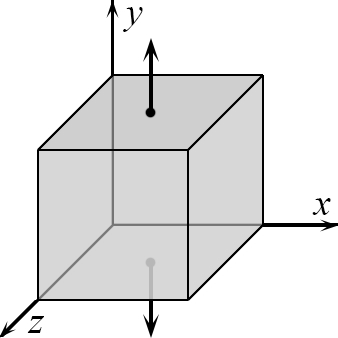
\includegraphics[width = 0.25\textwidth]{89-PS7-P3-NormalStress}	\qquad\qquad 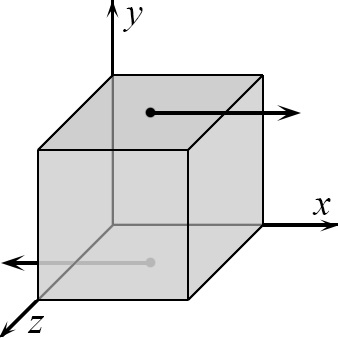
\includegraphics[width = 0.25\textwidth]{	89-PS7-P3-ShearStress}
	\caption{Left: A normal stress on the top/bottom faces.  Right:  A shear stress on the top/bottom faces.}
	\label{stresses}
	\end{figure}
	%~~~~~~~~~~~~~~ FIGURE ~~~~~~~~~~~~~~%

The \heavydef{stress tensor} $\stress$ is a type-(0,2) tensor whose components are these nine components.  That is, $\stress(\hat{e}_{i},\hat{e}_{j})$ gives
the $\hat{e}_{j}$-component of the force-per-unit-area acting on the face normal to the direction $\hat{e}_{i}$.  For example, $\stress(\hat{x},\hat{z})$ gives the
$z$-component of the force-per-unit-area acting on the right face (since the normal to the right face is in the $+\hat{x}$-direction).


\phline
%%%%%%%%%%%%%%%%%%%%%
\paragraph{(a)}		\extrapart
Suppose the stress tensor has components $\sigma_{ij}$.  Express the tensor $\stress$ as an expension in terms of its components and basis vectors/dual vectors/tensor products of
basis objects.  Let $\hat{n}$ be a unit vector.  Argue why $\stress(\hat{n},\cdot)$ is a dual vector.  Express this object in index notation.

\paragraph{}
\textit{Commentary:  We can interpret $\stress(\hat{n},\cdot)$ as a dual vector $\dual{F}$ that describes the force-per-unit-area on the cube face for which $\hat{n}$ is the 
normal vector.  Force is indeed most naturally interpeted as a dual vector since it can be defined via a gradient and gradients are most naturally dual vectors rather than 
vectors (we will see this when we introduce the Jacobian). Another way of seeing this?  The dual vector $\dual{F}$ eats a displacement vector $\vec{s}$ to give the
work done by the force, a scalar $W=\dual{F}(\vec{s})$.}

\phline
%%%%%%%%%%%%%%%%%%%%%
\paragraph{}
	%~~~~~~~~~~~~~~ FIGURE ~~~~~~~~~~~~~~%
	\setlength{\intextsep}{0pt}%
	\begin{wrapfigure}[8]{r}{0cm}
		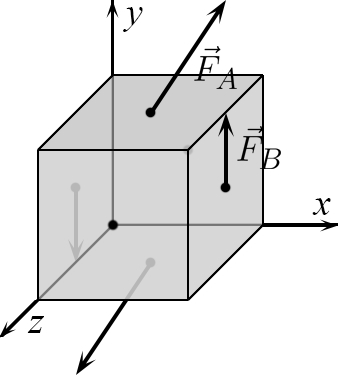
\includegraphics[width = 0.2\textwidth]{89-PS7-P3-StressedCube}
	\end{wrapfigure}
	%~~~~~~~~~~~~~~ FIGURE ~~~~~~~~~~~~~~%
Suppose our cube has uniform side-lengths $\ell$ and we apply forces as shown to the right to the cube.  The forces are 
$\dual{F}_{A} = (2f)\dual{\hat{x}} + (3f)\dual{\hat{y}}$ and 
$\dual{F}_{B} = (2f)\dual{\hat{y}}$, where $f$ is some constant with units of force and $\{\dual{\hat{x}},\dual{\hat{y}},\dual{\hat{z}}\}$ are the basis dual 
vectors.\footnote{We typically work with forces as vectors rather than dual vectors.  Really we can
consider $\vec{F}$ as the ``raised'' version of $\dual{F}$, with $F^{i} = g^{ij}F_{j}$.  Since we are typically working with Cartesian coordinates,
the components of the metric are the same as the components of the Kronecker delta and thus the vector and dual vector versions of force have the same components.} 


\paragraph{(b)}
Find the nine components of the stress tensor, $\sigma_{ij}$.  Arrange these components in the form of a matrix 
$\sigma^{\textrm{mat}}\equiv \begin{smpmatrix}{0.7} \sigma_{11} & \sigma_{12} & \sigma_{13}\\ \sigma_{21} & \sigma_{22} & \sigma_{23}\\ \sigma_{31} & \sigma_{32} & \sigma_{33}
\end{smpmatrix}$ where the first lower index `improperly' labels the row and the second lower index labels the column.
\spoilers{Your answer should be a symmetric matrix.}

\begin{solution}
	To find the components, we feed $\sigma$ the basis vectors. Just as the problem described, $\sigma(\hat{x},
	\hat{x})$ refers to the stress placed on the right face acting in the positive $\hat{x}$ direction. 
	Repeating this process for the remaining 8 basis vectors, we get:
	\[
		\sigma = \begin{pmatrix} 0 & 2f / \ell^2 & 0\\ 2f / \ell^2 & 3f / \ell^2 & 0\\ 0 & 0 & 0 \end{pmatrix} 
		= \frac{f}{\ell^2}\begin{pmatrix} 0 & 2 & 0\\ 2& 3& 0 \\0 & 0 & 0 \end{pmatrix} 
	\] 
\end{solution}
\phline
%%%%%%%%%%%%%%%%%%%%%%
\paragraph{}
Since we are in static equilibrium, we want the net \emph{torque} on our cube to be zero as well.  It turns out that this requirement implies that the stress tensor must
be \emph{symmetric}.

%%%%%%%%%%%%%%%%%%%%%%
\paragraph{(c)}		\extrapart
Show that the net torque for the setup from part (c) is indeed zero (take the pivot point to be the \emph{center} of the cube).  Consider a \emph{non}-symmetric
stress tensor $\sigma_{12}=p$ with all other components zero and show that the net torque is non-zero in this case.


\phline
%%%%%%%%%%%%%%%%%%%%%%
\paragraph{}
We can use the metric to raise the first index of $\sigma_{ij}$ to create an object $\widetilde{\stress}$ which is a linear transformation and whose components 
form a matrix.\footnote{What this linear transformation does is eat a unit vector and return the \emph{vector version} of the force acting on the plane normal to the unit vector,
$\vec{F}\equiv \tilde{g}(\dual{F})$.}
Since we are dealing with Cartesian coordinates in regular 3D space, it turns out that the matrix representation for $\widetilde{\stress}$ is the same
as the matrix you found part (b).  Since we are now dealing with a linear transformation, we can talk about eigenvalues and eigenvectors!

\paragraph{(d)}
Find the eigenvalues and eigenvectors of $\widetilde{\stress}$.  The eigenvalues are called the \heavydef{principal stresses}
and the planes normal to the eigenvectors are the \heavydef{principal planes}.  
\spoilers{In part (b) you should have found $\stress \doteq \frac{f}{\ell^{2}}\begin{smpmatrix}{0.8} 0 & 2 & 0 \\ 2 & 3 & 0 \\ 0 & 0 & 0 \end{smpmatrix}$, where the
entry in the $i$-th row and $j$-th column is the component $\sigma_{ij}$.}

\begin{solution}
	Building off part (b), we know that the matrix is:
	\[
		\tilde \sigma = \frac{f}{\ell^2}\begin{pmatrix} 0 & 2 & 0\\ 2 & 3 & 0 \\ 0 & 0 & 0 \end{pmatrix} 
	\] 
	Solving this matrix for eigenvalues and eigenvectors (I just used Mathematica for this since we've
	already had our homework on finding eigenvectors and eigenvalues) we get: 
	\begin{align*}
		\lambda_1 &= \frac{4f}{\ell^2}, \vec v_1 = \begin{pmatrix} 1 \\2\\0 \end{pmatrix} \\
		\lambda_2 &= -\frac{f}{\ell^2}, \vec v_2 = \begin{pmatrix} -2 \\ 1 \\0 \end{pmatrix} \\
		\lambda_3 &= 0, \vec v_3 = \begin{pmatrix} 0 \\ 0 \\ 1 \end{pmatrix}  
	\end{align*}
\end{solution}
%%%%%%%%%%%%%%%%%%%%%%
\paragraph{(e)}		\extrapart
Redraw the cube oriented so the six faces are parallel to the principal planes and draw in the forces/stresses on this new picture.\footnote{We can redraw the cube because we are 
really talking about infinitesimal volume elements of our object when we are talking stresses, 
so we can pick any cube orientation we want.}
Why will analyzing this system with this picture may be more straightforward than analyzing our original system?

\phline
 %%%%%%%%%%%%%%%%%%%%%%
\paragraph{(f)}
	%~~~~~~~~~~~~~~ FIGURE ~~~~~~~~~~~~~~%
	\setlength{\intextsep}{0pt}%
	\begin{wrapfigure}[7]{r}{0cm}
		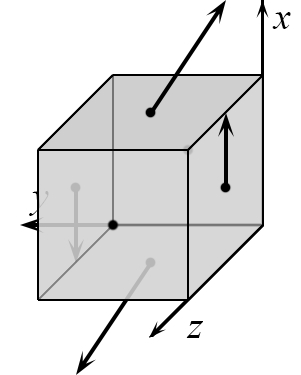
\includegraphics[scale=0.5]{89-PS7-P3-RotatedAxis}
	\end{wrapfigure}
	%~~~~~~~~~~~~~~ FIGURE ~~~~~~~~~~~~~~%
Suppose we performed a change-of-basis by rotating our basis vectors $90^{\circ}$ counterclockwise about the $\hat{z}$-axis, as shown to the right (while keeping the
actual stresses unchanged).
Based on this new picture, what are the new components of the stress tensor $\sigma_{[\textrm{new}]ij}$?  
Show that this is consistent with a passive transformation  of your answer from part (b) using the change-of-basis matrix 
$\mathsf{C} = \begin{smpmatrix}{0.7} 0 & -1 & 0 \\ 1 & 0 & 0 \\ 0 & 0 & 1 \end{smpmatrix}$.
\spoilers{The result from Problem 7.2(e) will be very useful here!}

\bigskip
\begin{solution}
	Working it out from the diagram using the same logic as we did in part (b), we get that the new stress 
	matrix is:
	\[
		\sigma_{[\text{new}]} = \frac{f}{\ell^2}\begin{pmatrix} 3 & -2 & 0 \\ -2 & 0 & 0 \\0&0&0 \end{pmatrix} 
	\] 
	We then use the fact that $\sigma_{[\text{new}]} = C^{-1} \sigma_{[\text{old}]} C$, and indeed doing this 
	matrix multiplication (done via computer) gives:
	\[
		\sigma_{\text{new}} = \frac{f}{\ell^2}\begin{pmatrix} 3 & -2 & 0\\ -2 & 0 & 0 \\ 0 & 0 &0 \end{pmatrix} 
	\] 
	which does match our desired result. 
\end{solution}
\bigskip
\dphline
\pagebreak
%%%%%%%%%%%%%%%%%%%%%%%%%%%%%%%%%%%%%%%%%%%%%%%%%%%%%%%%%%%%%%%%%%%%%%%%%%%%%%%%
\section*{7.4 - Strain and Stiffness}
\relevid{The Tensor Product; Contraction; Application - Rotational Dynamics}

\paragraph{}
In continuum mechanics, \heavydef{strain} is the measure of the relative deformation of a small element of material (such as our small cube of jello from the previous problem).
For example, if we were considering a 1D spring example of equilibrium length $\ell$ stretched an additional distance  $\Delta\ell$, then the strain of the spring would be the ratio 
$\Delta\ell/\ell$.  

\paragraph{}
For our 3D example, let $x_{0}$, $y_{0}$, and $z_{0}$ be the equilibrium lengths of our cube.  
There are many strains we can describe:  We can apply a \heavydef{normal strain} (a stretch or a compression) by stretching the \emph{right face} to the right by an amount 
$\Delta x$, as shown in the left figure in Fig.~\ref{strains} (the deformation is in the direction of the normal to the face).  
The value of this strain is expressed as the dimensionless ratio $\epsilon_{11} \equiv \Delta x/x_{0}$. 
We can also apply a \heavydef{shear strain} (a shearing of the cube) by sliding the \emph{top face} of the cube in to the right by an amount $\Delta x$, 
as shown in the right figure in Fig.~\ref{strains} (the deformation is in a direction perpendicular to the normal to the face).  
The value of this strain is expressed as the dimensionless ratio $\epsilon_{12} \equiv \Delta x/y_{0}$.
There are three possible strains (one normal, two shear) that we can apply to each of the three pairs of faces of the cube, for a total of nine strains.  Ooh, 
this \emph{also} looks like a tensor!
The \heavydef{strain tensor} $\boldsymbol{\epsilon}$ is a type-(0,2) tensor with components $\epsilon_{ij}$ defined to eat a vector and return a dual vector.
	\begin{itemize}
		\item The first index again tells you \emph{which face} of the cube you are looking at.
		\item The second index tells you about the \emph{components of the deformation}.
		\item Example: $\epsilon_{23}$ tells you that there is a deformation of the top face (which has normal vector $\hat{y}=\hat{e}_{2}$) in the direction of $\hat{z}=\hat{e}_{3}$.
		\item We take the strain tensor to be \emph{symmetric} in its two lower indices, $\epsilon_{ij} = \epsilon_{ji}$.  
	\end{itemize}

	%~~~~~~~~~~~~~~ FIGURE ~~~~~~~~~~~~~~%
	\begin{figure}[ht]	
	\centering
		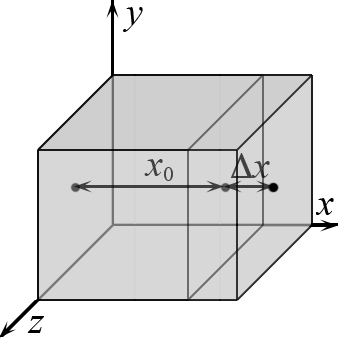
\includegraphics[width = 0.25\textwidth]{89-PS7-P4-NormalStrain}	\qquad\qquad 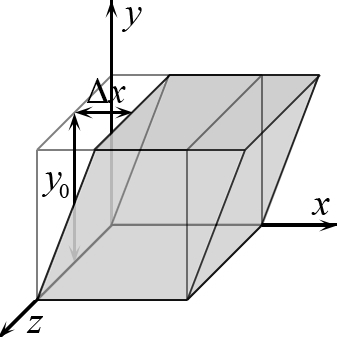
\includegraphics[width = 0.25\textwidth]{89-PS7-P4-ShearStrain}
	\caption{Left: A normal strain of the right/left faces.  Right:  A shear strain of the top/bottom faces faces.}
	\label{strains}
	\end{figure}
	%~~~~~~~~~~~~~~ FIGURE ~~~~~~~~~~~~~~%

\phline
%%%%%%%%%%%%%%%%%%%%%
\paragraph{}
Consider the strain tensor with components $\epsilon_{12} = \epsilon_{21} = a$ with all other components zero, where $a$ is some dimensionless small number.

\paragraph{(a)}		\extrapart
Describe the shape or sketch a picture of the cube under this strain.


%%%%%%%%%%%%%%%%%%%%%
\paragraph{(b)}
Write down the components of $\strain$ for the following deformations (you may arrange these components in a matrix, $\epsilon^{\mat}$ where component
$\epsilon_{ij}$ is the entry in the $i$-th row and $j$-th column):
	\begin{enumerate}
		\item  \heavydef{Not-for-credit example:}  The left- and right-sides of the cube are compressed inward by a fractional amount $\delta$.  
		The rest of the cube remains unchanged.
		\item  The left- and right-sides of the cube are compressed inward by a fractional amount $\delta$ and correspondingly the other four faces are bulged out
		by a fractional amount $\beta$.

			\begin{solution}
				Just as an example for the logic here, we have $\epsilon_{11}$ to be the strain in the $\hat{x}$
				direction on the right face, which we have is $-\delta$. Doing the same for the other 
				elements, we get:
				\begin{align*}
					\epsilon_{11} &= -\delta & \epsilon_{12} &= 0 & \epsilon_{13} &= 0 \\
						\epsilon_{21} &= 0 & \epsilon_{22} &= \beta & \epsilon_{23} &= 0\\
						\epsilon_{31} &= 0 & \epsilon_{22} &= 0 & \epsilon_{33}&= \beta
				\end{align*}
			\end{solution}
		\item  The left- and right-sides of the cube are compressed inward by a fractional amount $\delta$ and sheared by an equal amount upwards/downwards.

			\begin{solution}
				Here, we have to account for the fact that the net torque on the whole system is zero, so 
				there's actually another shear on the top and bottom faces to cancel out this torque. Applying 
				the same logic as before now, we get: 
				\begin{align*}
					\epsilon_{11}&= -\delta & \epsilon_{12} &= \delta & \epsilon_{13} &= 0\\
					\epsilon_{21} &= \delta & \epsilon_{22} &= 0 & \epsilon_{23} &= 0\\ 
					\epsilon_{31} &= 0 & \epsilon_{32} &= 0 & \epsilon_{33} &= 0
				\end{align*}
			\end{solution}
	\end{enumerate}
\note{Detailed solutions to the not-for-credit example (1) are given in the problem set supplement.}
\spoiler{Symmetry of the strain tensor means that the described strain in the setup (3) means that what is described isn't the \emph{only} deformation happening to the cube...}


\phline
%%%%%%%%%%%%%%%%%%%%%
\paragraph{}
The strain is connected to the stress via a form of \heavydef{Hooke's law} for elastic materials (in 1D this becomes $F=-k\Delta x$).  
To lowest order, this will be a linear relationship, so we have
	\begin{equation*}
		\stress = \stiffness\strain,
	\end{equation*}
where $\stiffness$ is the \heavydef{stiffness tensor} describing the various elastic properties of the material.  The combination $\stiffness\strain$ indicates some form of
tensor-product-and-contractions between the stiffness and strain tensors.

\paragraph{(c)}
Given that $\strain$ and $\stress$ are both type-(0,2) tensors, determine the possibilities for the tensor types of $\stiffness$.
Write out what Hooke's law would look like in \emph{component form} for each of these cases.  What units must the components of stiffness possess?

\begin{solution}
	Firstly, we note that any contraction within $C$ effectively means nothing, so this means that any 
	contraction that occurs must be between a basis vector of $C$ and one of $\epsilon$. This means that 
	for every basis vector we contract, we have to add another so that the balance of a (0,2) tensor on both 
	sides is restored. Ultimately, this means that there are three possibilities for $C$. C can either 
	be a type (0, 0) (a scalar), a type (1, 1), or a type(2, 2). Writing these out:
	\begin{itemize}
		\item Type (0, 0): $\sigma_{ij} = C \epsilon_{ij}$.
		\item Type(1, 1): $\sigma_{ij} = C^l_i \epsilon_{lj}$
		\item Type(2, 2): $\sigma_{ij} = C^{lm}_{ij} \epsilon_{lm}$
	\end{itemize}
	In terms of the units, we know that $\sigma$ is dimensionless and $\epsilon$ is also dimensionless, so 
	this means that $C$ must carry all the dimension, hence $C$ must have units of force/area.
\end{solution}

\phline
%%%%%%%%%%%%%%%%%%%%%
\paragraph{}
The inverse of Hooke's law may be written $\strain = \comply\stress$, where $\comply$ is known as the \heavydef{compliance tensor} and is of the same type as 
$\stiffness$.  Let's design a physical experiment in the lab to narrow down the choices of tensor type we found in the previous part:  we will put our cube in a vice
and apply an inward stress/pressure on the left- and right-faces.  That is, $\sigma_{11} = -P$ with all other components zero.

\paragraph{(d)}
For each of the three Hooke's laws from the previous part, determine which components of strain can be non-zero when the described stress is applied.  Intuitively,
how do you think an elastic object would respond to this strain?  Use this to determine which of the three laws is most appropriate and why.

\begin{solution}
	Naturally, when we compress the material on both sides, we expect the material to bulge out in the other 
	two axes. In other words, we expect $\epsilon_{22}$ and $\epsilon_{33}$ to be nonzero. If $S$ is a type
	(0, 0) tensor, this means that 
	\[
		\epsilon_{ij} = S \sigma_{ij}
	\] 
	meaning that $\epsilon_{11}$ is the only nonzero component. But this cannot be the case, since 
	we expect $\epsilon_{22}$ to be nonzero. 

	If $S$ is a type (1, 1) tensor, this means that:
	\[
		\epsilon_{ij} = S^l_i \sigma_{lj}
	\] 
	If we compute $\epsilon_{22}$ from this: 
	\[
		\epsilon_{22} = S^l_2 \sigma_{l2}
	\] 
	and since only $\sigma_{11} \neq 0$, then we're forced to also conclude that $\epsilon_{22} = 0$. Again, 
	this is impossible, so $S$ cannot be a type (1, 1) tensor either. As for the nonzero entries, we see
	that all entries which have $j = 1$ can be nonzero, which is to say that thee first column of $\epsilon$
	are the only entries that can be nonzero. 

	Finally, if $S$ is a type (2, 2) tensor:
	\[
		\epsilon_{ij} = S^{lm}_{ij} \sigma_{lm}
	\] 
	Here, the value of $\epsilon_{ij}$ is determined entirely by our tensor $S$, since for every entry 
	of $\epsilon$ we are summing over the entirety of $\sigma$. This is good, since it means that $\epsilon_{22}$
	can be nonzero. In fact, since $S$ can be chosen freely, all the components of $\epsilon$ can be nonzero.
\end{solution}

\phline
%%%%%%%%%%%%%%%%%%%%%
\paragraph{}
You should have found that the stiffness tensor must be a type-(2,2) tensor.  Due to the form of Hooke's law, the symmetry properties of the stress and strain tensors get
inherited by the stiffness tensor.  In particular,
	\begin{alignat*}{3}
		C^{ji}_{\phantom{ij}k\ell} &= C^{ij}_{\phantom{ij}k\ell}		\qquad&&\mbox{Symmetry in the two upper indices.}\\
		C^{ij}_{\phantom{ij}\ell k} &= C^{ij}_{\phantom{ij}k\ell}		\qquad&&\mbox{Symmetry in the two lower indices.}
	\end{alignat*}

\paragraph{(e)}
How many total components will a type-(2,2) tensor in 3D space have?  Given the symmetry in the two upper indices, show or argue that there are only six independent choices 
for the pair of indices $(ij)$ and similarly for $(k\ell)$.  How many independent components does this leave the stiffness tensor?
\note{For example, the pair $(ij) = (12)$ and $(ij) = (21)$ are \ul{not} independent since $C^{12}_{\phantom{12}k\ell} = C^{21}_{\phantom{12}k\ell}$.}
\spoilers{The six components are (11), (22), (33), (23), (13), (12).}

\begin{solution}
	In 2D space, we have 4 indices and 3 values to choose from for each index, so we have $3^4 = 81$ total 
	possible components. Now given the symmetry of the tensor, we find that the components $(i, j) = (k, \ell) = (1, 1), 
	(1, 2), (1, 3), (2, 2), (2, 3), (3, 3)$ are the only independent components, since all the other combinations
	of $i$ and $j$ are symmetric to one of these six pairs. Therefore, for each pair of indices, there are 
	only 6 independent parameters.

	In total, this leaves the stiffness tensor with $6 \times 6 = 36$ independent parameters. 
\end{solution}

\phline
%%%%%%%%%%%%%%%%%%%%%
\paragraph{}
The six possible pairs for the upper pair of indices $(ij)$ can act as a single row index and the
six possible pairs for the lower pair of indices $(k\ell)$ can act as a single column index, allowing us to express the stiffness tensor as a $(6\times 6)$
matrix.  We can similarly express the six independent components of the strain and stiffness tensors as six-component row vectors.  For example, $\stress\doteq \begin{pmatrix}
\sigma_{11} & \sigma_{22} & \sigma_{33} & \sigma_{23} & \sigma_{13} & \sigma_{12}\end{pmatrix}$.  This is known as the 
\heavydef{Voigt form} for stress, strain, and stiffness.\footnote{The compliance tensor in this case can also be written
as a $(6\times 6)$-matrix and can be found as the matrix inverse of the $(6\times 6)$ stiffness matrix.  See \url{https://en.wikipedia.org/wiki/Voigt_notation} for more.}
There is an additional symmetry that becomes apparent when we express the stiffness tensor in Voigt form which is that the $(6\times 6)$-stiffness matrix $\stiffness^{(\textrm{mat})}$ 
is a \emph{symmetric} matrix.

\paragraph{(f)}
Given this new symmetry, how many total independent components remain for the stiffness tensor?

\begin{solution}
	Written in this form, we essentially have a symmetric, $6 \times 6$ matrix, meaning that the total
	number of independent components is given by the formula for the number of free parameters in a 
	symmetric matrix of dimension $n$:
	\[
	N = \frac{n(n+1)}{2}
	\] 
	Since this matrix has $6$ rows and columns, we sub $n = 6$: 
	\[
	N = \frac{6 \times 7}{2} = 21
	\] 
	this formula is a general formula to find the number of independent parameters for any symmetric matrix, 
	so we plug in the dimension of 6 to get our answer.
\end{solution}

\phline
%%%%%%%%%%%%%%%%%%%%%
\paragraph{}
\heavydef{Isotropic} materials are characterized by properties which are independent of direction.  
Glass is an isotropic material, for example, but something like 
wood, which has a defined grain direction, is anisotropic.  
Isotropy and the symmetries of the stiffness tensor imply that stiffness must be a linear combination of $g^{ij}g_{k\ell}$ and 
$\delta^{i}_{k}\delta^{j}_{\ell} + \delta^{i}_{\ell}\delta^{j}_{k}$.  Thus, only \emph{two} free scalar parameters remain in the stiffness tensor:
	\begin{itemize} 
		\item $K$, the \heavydef{bulk modulus},
		\item $\mu$, the \heavydef{shear modulus}.
	\end{itemize}
In terms of these parameters, the components of the stiffness tensor are
	\begin{equation}
		C^{ij}_{\phantom{ij}k\ell} = (K-\fracsm{2}{3}\mu)\,g^{ij}g_{k\ell} + \mu(\delta^{i}_{k}\delta^{j}_{\ell} + \delta^{i}_{\ell}\delta^{j}_{k})
	\label{isotropic}
	\end{equation}

%%%%%%%%%%%%%%%%%%%%%
\paragraph{(g)}
An isotropic material undergoes a stress and experiences a strain $\epsilon_{12} = \epsilon_{21} = a$, $\epsilon_{22} = b$ (all other components are zero).  
Use Hooke's law and Eq.~\ref{isotropic} to determine the components of the stress tensor $\sigma_{ij}$.

\begin{solution}
	Hooke's law states:
	\[
		\sigma_{ij} = C^{lm}_{ij} \epsilon_{lm}
	\] 
	So expanding $C$ in terms of equation 3, we have:
	\begin{align*}
		\sigma_{ij} &= \left[\left(K - \frac{2}{3}\mu\right) g^{lm}g_{ij} + \mu(\delta^l_i \delta^m_j + \delta^l_j\delta^m_i)\right]\epsilon_{lm}\\
					&= \left( K - \frac{2}{3}\mu \right) g^{lm}g_{ij}\epsilon_{lm} + \mu\delta^l_i\delta^m_j \epsilon_{lm} + \mu \delta^l_j \delta^m_i \epsilon_{lm}	\\
					&= \left( K - \frac{2}{3}\mu \right) g^{lm} g_{ij} \epsilon_{lm}+ \mu(\epsilon_{ij} + \epsilon_{ji}) 
	\end{align*}
	And since we're working in cartesian space, the metric is the Kronecker delta:
	\[
		\sigma_{ij} = \left( K - \frac{2}{3}\mu \right) \delta^{lm}\delta_{ij}\epsilon_{lm} + \mu(\epsilon_{ij} + \epsilon_{ji})
	\] 
	Now we can start plugging in the indices for $i, j$. Note that since we know $\sigma$ is a symmetric matrix, 
	we only have to plug in $(i, j) = (1, 1), (1, 2), (1, 3), (2, 2), (2, 3), (3, 3)$. Plugging this in:
	\begin{align*}
		\sigma_{11} &= \left( K - \frac{2}{3}\mu \right) \delta^{lm}\epsilon_{lm} + \mu(\epsilon_{11} + \epsilon_{11}) = \left( K - \frac{2}{3}\mu \right) \epsilon_{22} = \left( K - \frac{2}{3}\mu \right) b\\
		\sigma_{12} &= \left( K - \frac{2}{3}\mu \right) \delta^{lm} \underbrace{\delta_{12}}_{= 0} \epsilon_{lm} + \mu(\epsilon_{12} + \epsilon_{21}) = 2 \mu \epsilon_{12} = 2a \mu = \sigma_{12} \\
		\sigma_{13} &= \left( K - \frac{2}{3} \mu\right) \delta^{lm} \underbrace{\delta_{13}}_{=0} + \mu(\underbrace{\epsilon_{13} + \epsilon_{31}}_{=0}) = 0 + 0 = 0= \sigma_{31} \\
		\sigma_{22} &= \left( K - \frac{2}{3}\mu \right) \delta^{lm} \epsilon_{lm} + \mu(\epsilon_{22} + \epsilon_{22}) = \left( K - \frac{2}{3}\mu \right) \epsilon_{22} + 2 \mu \epsilon_{22} = b\left( K + \frac{4}{3}\mu \right) \\
		\sigma_{23} &= \left( K - \frac{2}{3}\mu \right) \delta^{lm} \underbrace{\delta_{23}}_{=0} \epsilon_{lm} + \mu(\underbrace{\epsilon_{23} + \epsilon_{32}}_{ = 0}) = 0 + 0 = 0 = \sigma_{32} \\
		\sigma_{33} &= \left( K - \frac{2}{3}\mu \right) g^{lm} \epsilon_{lm} = b\left( K - \frac{2}{3}\mu \right) 
	\end{align*}
	The other components of $\sigma$ are automatically determined from this, due to the symmetry. 
\end{solution}
\bigskip
\dphline
\pagebreak
%%%%%%%%%%%%%%%%%%%%%%%%%%%%%%%%%%%%%%%%%%%%%%%%%%%%%%%%%%%%%%%%%%%%%%%%%%%%%%%%
\section*{7.5 - Spherical Coordinates}
\relevid{The Metric;
The Jacobian and Coordinate Changes}

\paragraph{}
When we have a tensor field (a tensor that depends on where you are in space), we can do a coordinate change from old coordinates $\{x^{i}\}$ to new
coordinates $\{\tilde{x}^{i}\}$ by defining the \heavydef{Jacobian matrix} and the \heavydef{inverse Jacobian matrix},
	\begin{equation*}
		J^{i}_{\phantom{i}j} \equiv \pdiff{x^{i}}{\tilde{x}^{j}},	\qquad	(J^{-1})^{i}_{\phantom{i}j} \equiv	\pdiff{\tilde{x}^{i}}{x^{j}}.
	\end{equation*}
Upon a change-of-coordinates, {contravariant} indices (upper indices) transform via $\mathsf{J}^{-1}$ and {covariant} indices (lower indices) transform
via $\mathsf{J}$.
Consider the transformation from Cartesian coordinates $\smthreevect{x}{y}{z}$ to spherical polar coordinates $\smthreevect{r}{\theta}{\varphi}$.  Remember that the
\emph{physicist's} way of defining spherical coordinates has $\theta$ as the polar angle and $\varphi$ as the azimuthal angle,
	\begin{align*}
		x &= r\sin\theta\cos\varphi\\
		y &= r\sin\theta\sin\varphi\\
		z &= r\cos\theta.
	\end{align*}
In Cartesian coordinates the components of the metric tensor are $g_{ij} = \delta_{ij}$.

%%%%%%%%%%%%%%%%%%%%%
\paragraph{(a)}
Find the Jacobian matrix $\mathsf{J}$.
\extrasubpart{Compute the inverse of the Jacobian $\mathsf{J}^{-1}$.}

\begin{solution}
	Taking the derivatives, we get:
	\begin{align*}
		J^1_1 &= \sin \theta \cos \phi & J^1_2 &= r\cos \theta \cos \phi & J^1_3 &= -r \sin \theta \sin \phi\\
		J^2_1 &=  \sin \theta \sin \phi & J^2_2 &= r \cos \theta \sin \phi & J^2_3 &= r \sin \theta \cos \phi\\
		J^3_1 &= \cos \theta & J^3_2 &= -r \sin \theta & J^3_3 &= 0
	\end{align*}
	Arranging this into a matrix, we get:
	\[
		J = \begin{pmatrix} \sin \theta \cos \phi & r \cos \theta \cos \phi & -r \sin \theta \cos \phi\\
		\sin \theta \sin \phi & r \cos \theta \sin \phi & r \sin \theta \cos \phi \\
	\cos \theta & -r \sin \theta & 0\end{pmatrix} 
	\] 
\end{solution}
\phline
%%%%%%%%%%%%%%%%%%%%%
\paragraph{(b)}
Use the Jacobian matrix to find the components of the metric tensor in spherical coordinates.  You may put the components
of the type-(0,2) metric tensor in matrix form, $g^{\mat} = \begin{smpmatrix}{0.7} g_{rr} & g_{r\theta} & g_{r\varphi} \\
g_{\theta r} & g_{\theta\theta} & g_{\theta\varphi} \\ g_{\varphi r} & g_{\varphi\theta} & g_{\varphi\varphi}\end{smpmatrix}$.\medskip

\begin{solution}
	We have the relation that $g^{\text{mat}}_{\text{new}} = J^\top g^{\text{mat}}_{\text{old}} J$. Since
	the old basis was Cartesian, we know that $g^{\text{mat}}_{\text{old}} = \delta_{ij} = \mathbbold 1$. 
	Therefore, we find that $g^{\text{mat}}_{\text{new}} = J^\top J$. Computing this matrix multiplication
	using a computer, we get:
	\[
		g^{\text{mat}}_{\text{new}} = J^\top J = \begin{pmatrix} 1 & 0 & 0\\ 0 & r^2 & 0\\ 0 & 0 & r^2 \sin^2 \theta \end{pmatrix} 
	\] 
\end{solution}
\phline
%%%%%%%%%%%%%%%%%%%%%
\paragraph{(c)}
Given a vector $\vec{v} = v^{r}\hat{r} + v^{\theta}\hat{\theta} + v^{\varphi}\hat{\varphi}$, find the components $\tilde{v}_{i} \equiv g_{ij}v^{j}$ of the dual vector
$\underline{v}$ in spherical coordinates.

\begin{solution}
	Just working through it by plugging in the indices:
	\begin{align*}
		\tilde v_1 &= g_{1j}v^j =  v^r\\
		\tilde v_2 &= g_{2j}v^j = r^2 v^\theta\\
		\tilde v_3 &= g_{3j}v^j = r^2 \sin^2 \theta v^\phi
	\end{align*}
	and we're done!
\end{solution}

\paragraph{}
\textit{Commentary:  The above part shows that in other coordinate systems or with non-trivial metrics, we can't just ``transpose'' our vector to find a dual vector!}

\endofhomework
\addfooter
%%%%%%%%%%%%%%%%%%%%%%%%%%%%%%%%%%%%%%%%%%%%%%%%%%%%%%%%%%%%%%%%%%%%%%%%%%%%%%%%
\end{document}


